% !TEX root = main.tex
\section{Design Motivation}
\label{sec:design_motivation}
The goal of the proposed system is to demonstrate a radio communication system with adaptable sound quality. This main goal is the background for all design choices that is made. In this section, the motivation behind the key specifications and some of the solutions described in section \ref{sec:design_description} is given.

\subsection{System specifications}
\subsubsection{Transmit Power}
As shown in table \ref{tab:link_budget}, the transmitter PA power, $P_{PA}$, is set to \paPower dBm. As the purpose of the system is to demonstrate the adaptable quality feature, the transmit power was tuned to a value suitable for this purpose. Too high transmit power would give a received $E_b/N_0$ high enough to always transmit at the best quality, thus disabling us from demonstrating the quality adoption. 

\subsubsection{Modulation Scheme}
The system uses QPSK for low data rate transmission and QAM-16 for high data rate transmission. QPSK has the advantage of constant symbol amplitude and therefore reduces nonlinear effects in the amplifiers. Because of the orthogonality between the I and Q signals, QPSK also gives twice the capacity as BPSK for same $E_b/N_0$ sensitivity. QAM-16 is chosen for high data rates because the information content in each symbol is twice as big as for QPSK, making the difference big enough to demonstrate an audible effect.

\subsubsection{Bandwidth}
The motivation behind the adaptable quality feature, is to maximise data rate, for fixed bandwidth and transmit power. To demonstrate this feature, the system is designed width a fixed bandwidth, equal for both quality levels. The specific value for the bandwidth is however not important for this demonstration. The transmitted symbol rate is chosen large enough to enable both QPSK and QAM-16 transmission. The ideal Nyquist bandwidth is calculated from the symbol rate and the properties of the pulse shaping filter, and presented in table \ref{tab:link_budget}. 

%\subsubsection{Training Sequence}
%Barker codes is chosen as training sequence because it is the unique sequence with ideal autocorrelation property \cite{barker}. A total length of 26 training symbols is chosen to make the

 
\subsection{System Architecture}
The adaptable quality feature requires some additional logic, compared to a system without a feedback path. One important design choice is to determine where the decision of changing quality level (referred to as \textit{state}) is to be made. During the design of the proposed system, two solutions were considered:
\begin{enumerate}
\item 
The receiver decides when to change state and sends a simple message to the transmitter, telling it to change state. The receiver has its own state variable, and updates it after sending the message to the transmitter.

The advantage of this solution is that the receiver always know how the received symbols are modulated. Thus, no state information is needed in the transmitted packet. 

The draw back is that there will be some delay from the receiver ask for a change of state, until state change is completed. This will either cause a few packets to get lost in the meantime, or extra logic must be implemented to handle the issue. Extra logic must also be implemented to handle the case of bit errors in the ``change-state-message''.

\item
The transmitter decides when to change state and the receiver continuously send information about detected error rate to the transmitter. This requires information about the state to be contained in the data packet and the receiver will need more complexity in order to determine the incoming modulation format. 
However, this will eliminate the senario when the transmitter and the receiver are in different states. 
\end{enumerate}
We chose to implement the second solution. The state information is kept in the two different Barker sequences. Because we would have to search for one Barker sequence in the frame synchronisation anyway, searching for one more would be both computationally fast and easy to implement. In addition, the good autocorrelation properties of the Barker sequence makes the state information robust against noise, and no extra FEC is needed to keep this information safe. 

\subsection{Implemented Functionality}
\subsubsection{Source Enconding}
We chose not to implement any source encoding except for the primitive reduction of data rate. A source encoder removes redundancy in the speech data and increase the information content of every transmitted symbol. This functionality is not necessary to demonstrate the adaptable quality and is therefore not implemented. 

The source encoder also makes the system more sensitive to bit errors, as the information content in each bit is increased. Our system is designed to operate at $E_b / N_0$ low enough to demonstrate the quality adaption. When the received $E_b / N_0$ falls low enough to make the system change from QAM-16 to QPSK modulation, we would like the system to have a large margin before the BER for QPSK also get too high and the link is broken. Using a source encoder would make this window smaller and the system would be harder to demonstrate. 

\subsubsection{Scrambler}
Analysis of the received constellation diagram clearly showed that some symbols occurred more frequently at the receiver than others. Both the RF hardware and the pulse align algorithm are highly sensitive unequal energy distribution between I and Q. When comparing the received constellation from speech data to the constellation from random data, we could see that the quality was considerably increased when transmitting white data. We therefore implemented a scrambler to whiten the speech data before transmission. 

\subsubsection{FEC}
The implemented FEC algorithm is Hamming(7,4) and serves two purposes. In the data path, the receiver must estimate the number of bit errors and send this number back to the transmitter. In the BER path, the transmitter use the FEC to determine if the received BER packet is valid or not. If the number of bit errors in the BER packet is above a predefined threshold, the packet is considered as invalid in order to reduce the risk of undesired changes of quality level. 

This particular algorithm was chosen for its simplicity and decent trade-off between redundancy overhead and minimal Hamming distance. The algorithm allows for detection of any two-bit errors in every 7 bit code word, which was considered sufficient for this purpose. In addition, pre-written C-code implementation exists \cite{hamming} which saved development time. More advanced FEC algorithms should be considered for applications where bandwidth limitations require less overhead, or error correction is necessary. 

\subsubsection{Frequency and Phase Synchronisation}
The Mth-power algorithm is chosen for frequency synchronisation because of the good accuracy and simple implementation. By estimating the frequency offset as the mean of the angular deviation between all consecutive symbols, the ML estimate of the frequency offset is obtained. In addition, the Mth-power algorithm does not require a known training sequence, and may be applied to all data samples when QPSK modulation is being used. By extending the algorithm to a Kalman filter, the mean square error between the estimated offset and the actual offset is minimised. The improvement from the Kalman filter is clearly seen in figure \ref{fig:kalman_freq} which shows the estimated frequency offset at the receiver with and without Kalman filter.

\begin{figure}[htbp]
\centering
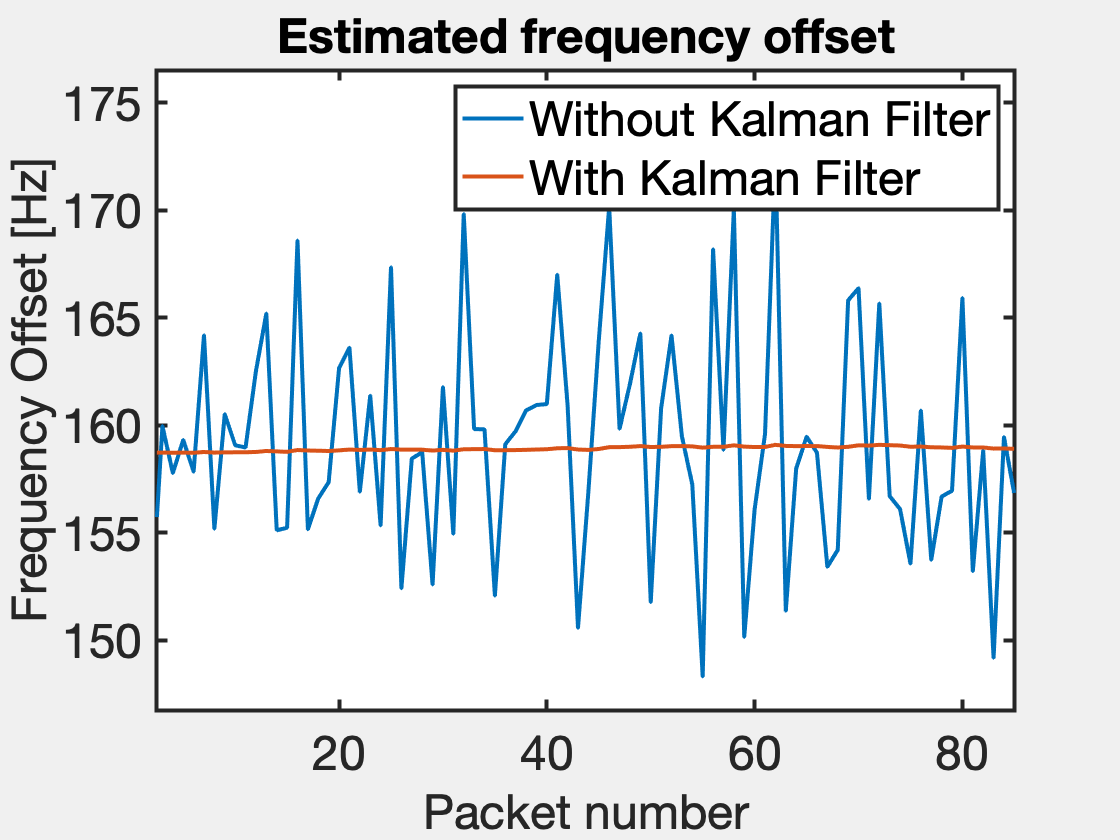
\includegraphics[width=\figW\linewidth]{KalmanFreq.png}
\caption{Estimated frequency offset with and without Kalman filter}
\label{fig:kalman_freq}

\end{figure}

The Mth-power algorithm is however not linear, making it less suited for phase estimation. Therefore, the linear algorithm based on comparing the phase directly to the training sequence is used for estimating the phase.
 





